\documentclass[ngerman,aspectratio=169]{beamer}
\usepackage[utf8]{inputenc}

\usepackage[binary-units=true]{siunitx}
\usepackage[german=quotes]{csquotes}
\usepackage[nooldvoltagedirection]{circuitikz}
\usepackage[outline]{contour}
\usepackage[shorthands=off,ngerman]{babel}
\usepackage[style=iso-numeric,minnames=1,maxnames=3,giveninits,uniquename=init]{biblatex}
\usepackage[T1]{fontenc}
\usepackage{adjustbox}
\usepackage{amsmath}
\usepackage{booktabs}
\usepackage{caption}
\usepackage{datetime}
\usepackage{environ}
\usepackage{fontawesome5}
\usepackage{graphicx}
\usepackage{hyperref}
\usepackage{pgfplots}
\usepackage{spreadtab}
\usepackage{tabularx}
\usepackage{textcomp}
\usepackage{tikz}
\usepackage{xcolor}

\addbibresource{references.bib}
\captionsetup{justification=centering,font=footnotesize}
\contourlength{0.7pt}
\graphicspath{{images/}}
\pgfplotsset{width=9cm,compat=newest}
\setlength{\bibhang}{0cm} % left-align bibliography
\sisetup{locale = DE}
\tikzset{>=Stealth}
\usetheme{metropolis}
\usetikzlibrary{angles,arrows.meta,,calc,math,positioning,shadows,trees,quotes}
\tikzset{
  invisible/.style={opacity=0},
  visible on/.style={alt={#1{}{invisible}}},
  alt/.code args={<#1>#2#3}{%
    \alt<#1>{\pgfkeysalso{#2}}{\pgfkeysalso{#3}} % \pgfkeysalso doesn't change the path
  },
}

\title{Passive Radar}
\subtitle{Grundlagen der Signalverarbeitung}
\date{Jannuar 2021}
\author{Andreas Baulig}
\institute{Hochschule Esslingen}
\logo{
\includegraphics[height=1cm]{hs-esslingen_logo.png}}

\newcommand{\nologo}{\setbeamertemplate{logo}{}}

\begin{document}

\frame{\titlepage}

{
  \nologo{}
  \begin{frame}[allowframebreaks]
    \frametitle{Agenda}
    \tableofcontents
  \end{frame}

  % !TeX root = ../../beamer.tex
\section{Was ist Passiv Radar}

\begin{frame}
    \frametitle{Was ist Radar}

    \begin{columns}
        \begin{column}{0.6\textwidth}
            \begin{itemize}
                \item \textbf{RA}dio \textbf{D}etection and \textbf{R}anging
                \item Messung von \textbf{Entfernung} und \textbf{Geschwindigkeit}
                      \begin{itemize}
                          \item<3-> Zeitversatz \(\tau\)
                          \item<3-> Frequenzversatz \(f_{d}\)
                      \end{itemize}
            \end{itemize}
        \end{column}
        \begin{column}{0.4\textwidth}
            \begin{figure}
                \centering
                \begin{tikzpicture}
                    
\def\tickamp{0.025cm}
\def\tickseg{0.5cm}
\node [label={below:Radar}] (radar) at (0,0) {\Huge\faSatelliteDish};

\node [label={above:Target}] (target) at (3,3) {\Huge\faPlane};

\draw [visible on=<1>,decorate,decoration={expanding waves,angle=6,segment length=3pt},blue!60] (radar) -- node [fg] {\small\contourlength{2pt}\contour{bg}{Pulse}} (target);

\draw [visible on=<2->,decorate,decoration={expanding waves,angle=60,segment length=6pt},red!60] (target) -- node [fg] {\small\contourlength{2pt}\contour{bg}{Echo}} (radar);

                \end{tikzpicture}
            \end{figure}
        \end{column}
    \end{columns}
\end{frame}

\begin{frame}
    \frametitle{Was heißt Passiv?}

    \begin{columns}
        \begin{column}{0.6\textwidth}
            \begin{itemize}
                \item Beleuchtung durch Sender in der \textbf{Umgebung}
                \item Operator hat \textbf{keine Kontrolle} über Beleuchter
                \item Beleuchter und Empfänger sind \textbf{räumlich getrennt}
            \end{itemize}
        \end{column}
        \begin{column}{0.4\textwidth}
            \begin{figure}
                \centering
                \resizebox{\linewidth}{!}{
                    \begin{tikzpicture}
                        \newcommand\drawTopology[4]{
    \coordinate (rx1_coord) at (-2,0);
    \coordinate (tx1_coord) at (2,0);
    \coordinate (target_coord) at (1.25,3);

    \node at (tx1_coord) [text width=0.5cm,text height=1cm] (tx) {};
    \node at (tx1_coord) [antenna,scale=0.5,below=-0.5cm] {};
    \path let \p1=(tx.north west), \p2=(tx.south east), \p3=(tx) in [label={below:Receiver}] ({\x3-0.4cm},\y1) rectangle ({\x3+0.4cm},\y2) node [below] at (\x3,\y2) {Illuminator};

    \node at (rx1_coord) [text width=0.5cm,text height=0.75cm] (rx) {};
    \node at (rx1_coord) [antenna,scale=0.5,below=-0.5cm] {};
    \path let \p1=(tx.north west), \p2=(tx.south east), \p3=(rx) in [label={below:Receiver}] ({\x3-0.4cm},\y1) rectangle ({\x3+0.4cm},\y2) node [below] at (\x3,\y2) {Receiver};

    \node at (target_coord) [label={above:Target}] (target) {\Huge\faPlane};

    \draw [visible on={#1},decorate,decoration={expanding waves,angle=35,segment length=4pt},blue!60] (tx) -- (target);
    \draw [visible on={#2},decorate,decoration={expanding waves,angle=25,segment length=4pt},red!60] (target) -- node [#4] {\small\contourlength{2pt}\contour{#3}{Echo}} (rx);
    \draw [visible on={#1},decorate,decoration={expanding waves,angle=15,segment length=4pt},blue!60] (tx) -- node [#4] {\small\contourlength{2pt}\contour{#3}{Reference}} (rx);
}

                        \drawTopology{<2->}{<3->}{bg}{fg}
                    \end{tikzpicture}
                }
            \end{figure}
        \end{column}
    \end{columns}
\end{frame}

\begin{frame}
    \frametitle{Beleuchtungsquellen (Illuminators of Opportunity)}

    \begin{columns}
        \begin{column}{0.2\textwidth}
            \begin{figure}
                \raggedleft{}
                \begin{tikzpicture}
                    \begin{axis}[
                            ymode=log,
                            height=6cm,
                            width=2cm,
                            hide x axis,
                            axis y line=left,
                            ymin=1,
                            ymax=100,
                            ylabel={Entfernung [\si{\kilo\metre}]},
                        ]
                        \addplot [draw=none] {1};
                    \end{axis}
                \end{tikzpicture}
            \end{figure}
        \end{column}
        \begin{column}{0.8\textwidth}
            \begin{itemize}
                \item FM-Radio
                \item DVB-T (Digitales Fernsehen)
                \item DAB (Digitales Radio)
                \item LTE
                \item GSM
                \item WiFi
            \end{itemize}
        \end{column}
    \end{columns}
\end{frame}

  % !TeX root = ../../beamer.tex
\section{Geschichte}

\begin{frame}
    \frametitle{Das Daventry Experiment}

    \begin{columns}
        \begin{column}{0.5\textwidth}
            \begin{itemize}
                \item \textbf{Passives} Radar
                \item BBC Sendeturm als Beleuchter
                \item Detektion von Bomber-Flugzeug
            \end{itemize}
        \end{column}
        \begin{column}{0.5\textwidth}
            \begin{figure}
                \centering
                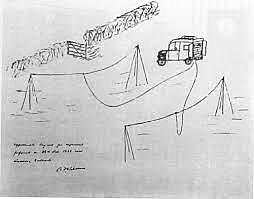
\includegraphics[height=5cm]{daventry_experiment.jpg}
                \caption{Skizze des Daventry Experiments von 1935~\cite{WattsonWatt1935}.}
            \end{figure}
        \end{column}
    \end{columns}
\end{frame}

\begin{frame}
    \frametitle{Chain Home}

    \begin{columns}
        \begin{column}{0.5\textwidth}
            \begin{itemize}
                \item Aktives Radar
                \item Nutzung während des 2. Weltkriegs
                \item Frühwarnradar gegen deutsche Luftangriffe
                \item Erste Inbetriebnahme 1937
            \end{itemize}
        \end{column}
        \begin{column}{0.5\textwidth}
            \begin{figure}
                \centering
                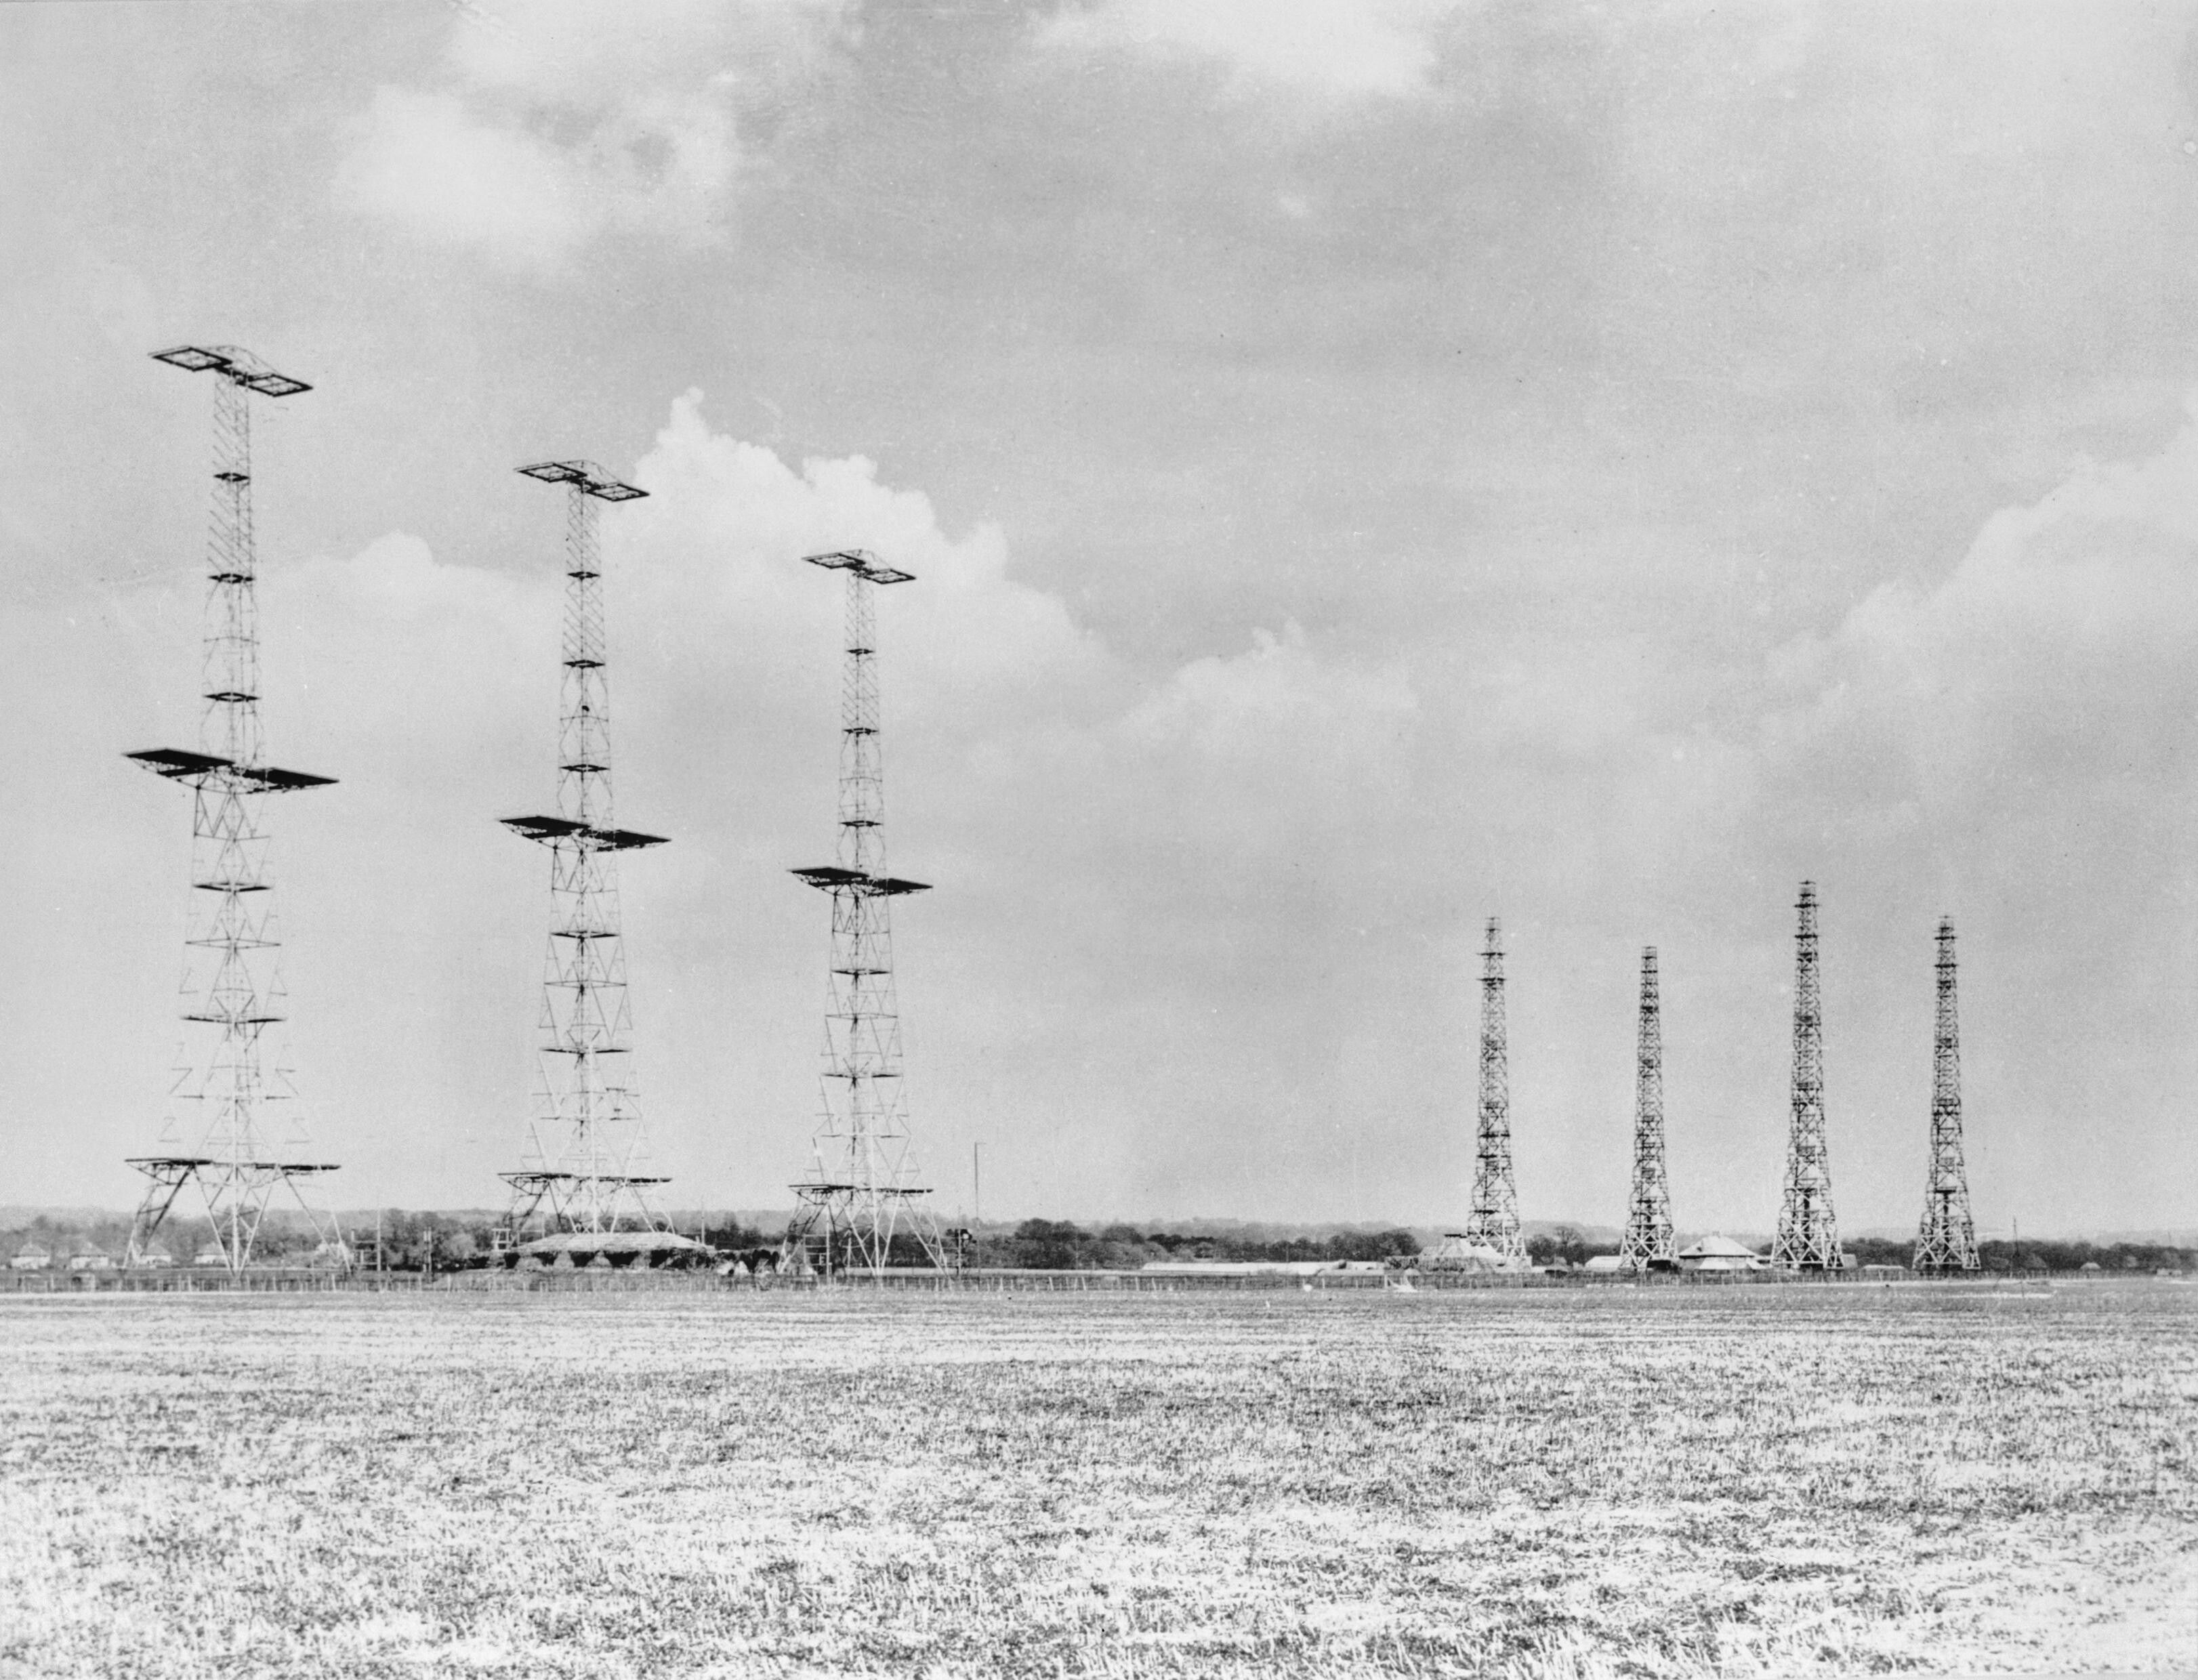
\includegraphics[height=5cm]{chain_home.jpg}
                \caption{Chain Home Antennen der Royal Airforce. Foto 1945~\cite{RoyalAirForce1945}.}
            \end{figure}
        \end{column}
    \end{columns}
\end{frame}

\begin{frame}
    \frametitle{Klein Heidelberg}

    \begin{columns}
        \begin{column}{0.44\textwidth}
            \begin{figure}
                \centering
                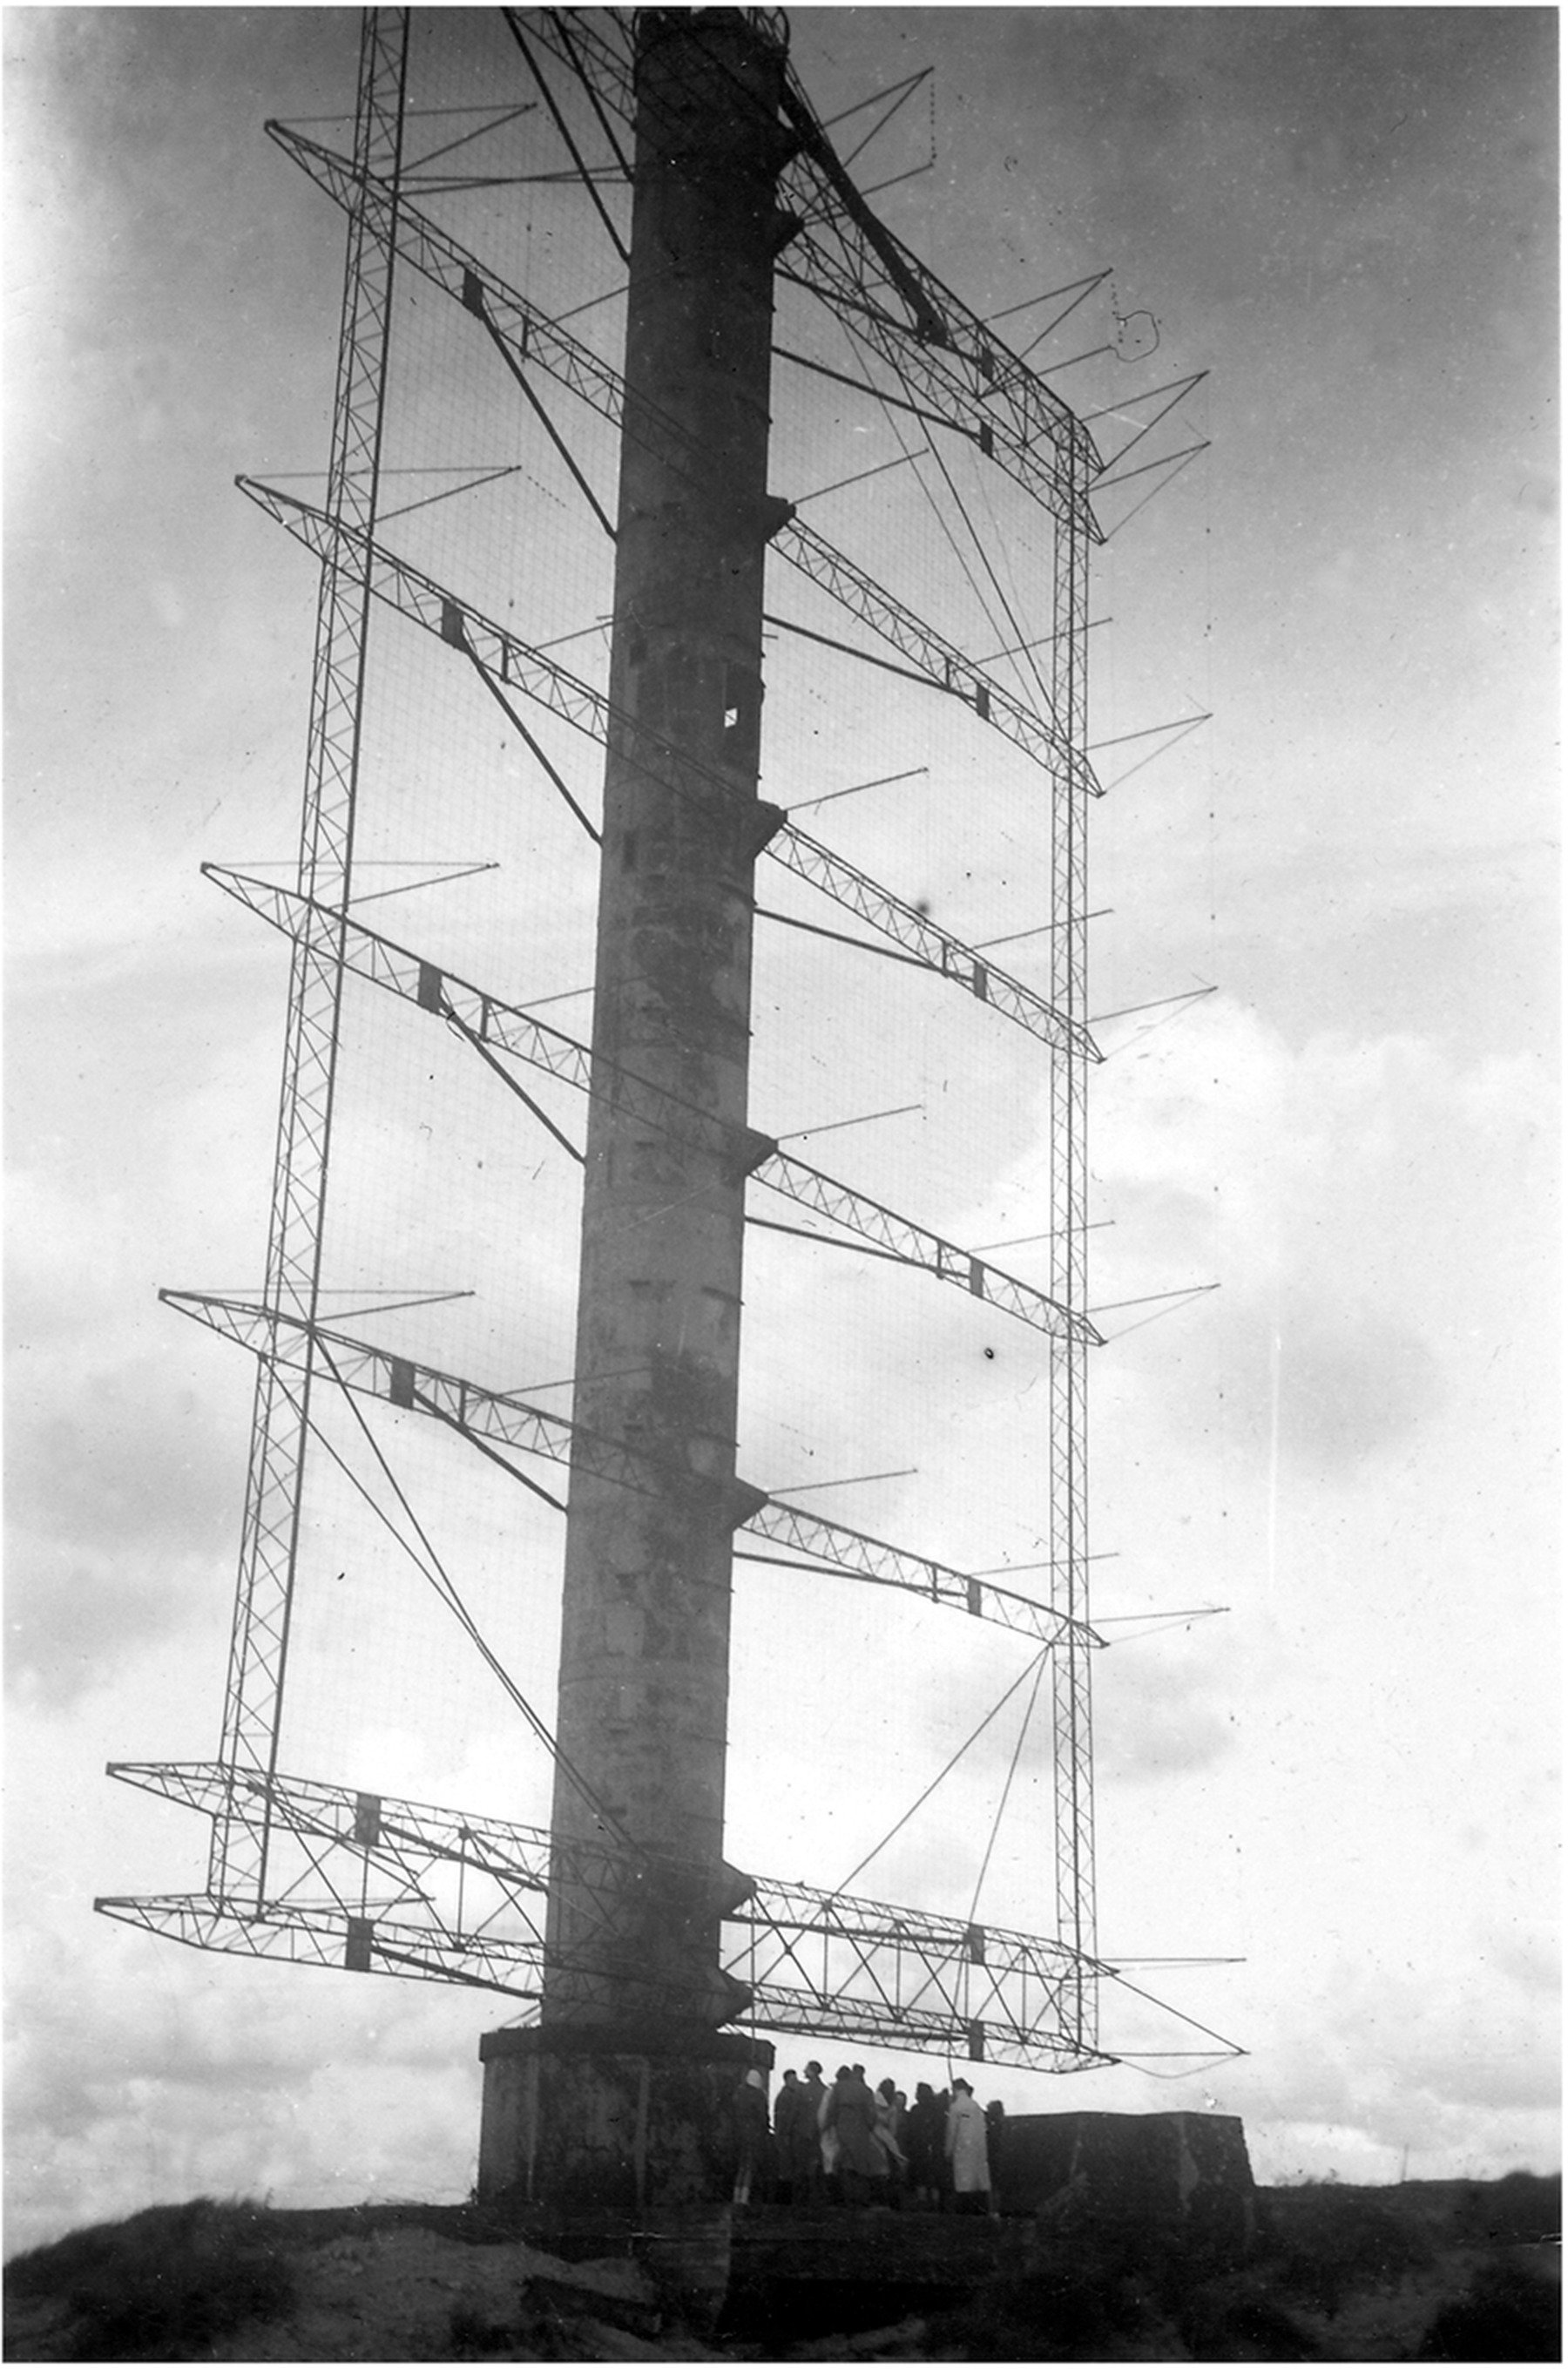
\includegraphics[height=4.5cm]{klein_heidelberg.jpg}
                \caption{Antenne des Klein Heidelberg Empfängers BIEBER (Oostvoorne, NL). Foto 1947~\cite{Rijpsma2005} as cited in~\cite{Griffiths2010}.}
            \end{figure}
        \end{column}
        \begin{column}{0.56\textwidth}
            \begin{itemize}
                \item \textbf{Passives} Radar
                \item Detektion von britischen Bombern über dem Ärmelkanal
                \item Nutzte \textbf{britisches Chain-Home} als Beleuchter
                \item Fertigstellung 1942
            \end{itemize}
        \end{column}
    \end{columns}
\end{frame}

\begin{frame}
    \frametitle{Neuzeit}

    \begin{columns}
        \begin{column}{0.55\textwidth}
            \begin{figure}
                \centering
                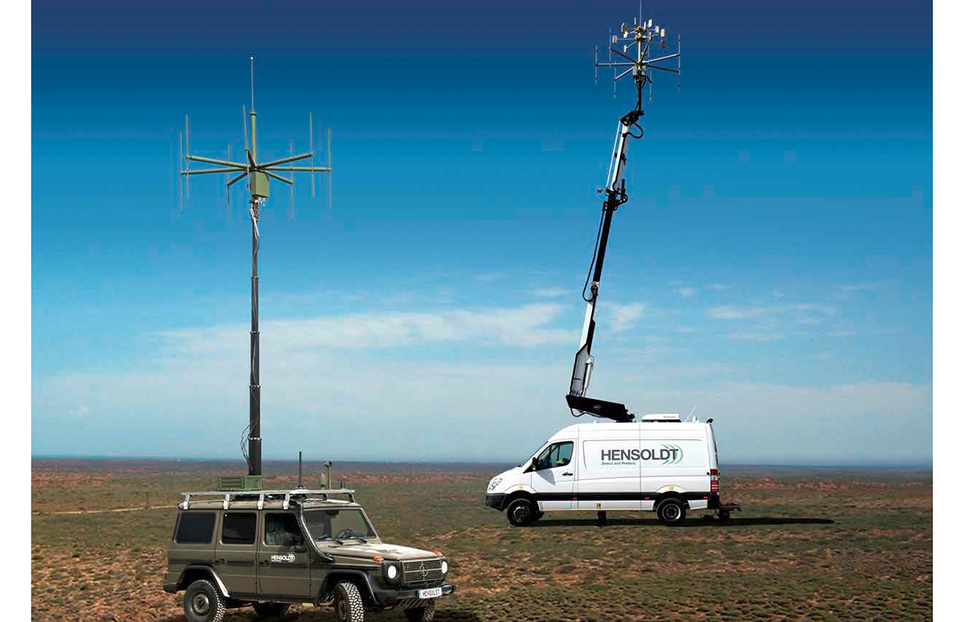
\includegraphics[height=4.75cm]{twinvis.png}
                \caption{TwInvis®. Modernes Passivradarsystem des Unternehmens Hensoldt~\cite{Hensoldt2019}.}
            \end{figure}
        \end{column}
        \begin{column}{0.45\textwidth}
            \begin{itemize}
                \item Zunächst basierend auf FM Beleuchtern
                \item Später DAB und DVB-T
                \item GSM, LTE
                \item \dots
            \end{itemize}
        \end{column}
    \end{columns}
\end{frame}

  % !TeX root = ../../beamer.tex
\section{Bistatisches Prinzip}

\begin{frame}
    \frametitle{Monostatische Geometrie}

    \begin{figure}
        \centering
        \begin{tikzpicture}
            \coordinate (horizon) at (3,0);

            \begin{scope}
                \clip (0,0) rectangle ({sqrt(2*pow(3,2))},{sqrt(2*pow(3,2))});
                \draw (0,0) circle [radius={sqrt(2*pow(3,2))}];
            \end{scope}

            \node [label={below:Radar}] (radar) at (0,0) {\Huge\faSatelliteDish};

            \node [label={above:Target}] (target) at (3,3) {\Huge\faPlane};

            \draw [<->,red] (radar) -- (target);
            \draw [dotted] (radar) -- (horizon);

            \pic [draw,angle radius=1.5cm,angle eccentricity=0.8,"$\phi$"] {angle=horizon--radar--target};
        \end{tikzpicture}
        \caption{Monostatische Geometrie bei konventionellem Radar.}
    \end{figure}
\end{frame}

\begin{frame}
    \frametitle{Bistatische Geometrie}

    \begin{figure}
        \centering
        \resizebox{0.7\textwidth}{!}{
            \begin{tikzpicture}
                % !TeX root = ../main.tex
\coordinate (rx1_coord) at (-2,0);
\coordinate (tx1_coord) at (2,0);
\coordinate (target_coord) at (1,1.25);

\node at (tx1_coord) [draw,fill=white] (tx1) {Tx};

\node at (rx1_coord) [draw,fill=white] (rx) {Rx};

\begin{scope}
    \clip
    let
    \p1=(target_coord),
    in
    (\x1 - 0.75cm,\y1 + 0.75cm) rectangle +(1.5,-1.5);
    \draw [color=gray]
    (2.42539052968,0) arc [start angle=0,end angle=360,x radius=2.42539052968,y radius=1.37204927807];
\end{scope}

\node at (target_coord) [label={[fill=white]above:Target}] (target) {\faPlane};

\draw [->,color=red] (tx1) -- node [black,midway,right,align=center] {$R_1$} (target);
\draw [->,color=red] (target) -- node [black,midway,left=4pt,align=center] {$R_2$} (rx);
\draw [->,color=blue] (tx1) -- node [black,midway,below,align=center] {$R_{\text{b}}$} (rx);

\pic [draw,angle radius=1cm,"$\beta$"] {angle=rx1_coord--target_coord--tx1_coord};

                \drawBistaticGeometry{bg}
            \end{tikzpicture}
        }
        \caption{Baseline \(R_{\text{b}}\), Entfernung: Sender/Ziel \(R_{1}\), Entfernung: Ziel/Empfänger \(R_{2}\), Bistatischer Winkel \(\beta\), Bewegungsrichtung Ziel \(\delta\), Geschwindigkeitsvektor \(v\).}
    \end{figure}
\end{frame}


  \begin{frame}[allowframebreaks]
    \frametitle{Quellen}
    \printbibliography
  \end{frame}
}

\end{document}
